\chapter{Алгоритм построения маршрутов}

\section{Модели данных}
В этом разделе будут описаны 3 способа представления данных о транспортной системе в виде графа, на котором впоследствии будут применятся алгоритмы для построения маршрутов и доступ к которому будет иметь построитель маршрутов.
\subsection{Статичный граф}
В статичном случае каждое ребро взвешенно функцией $c:E \rightarrow R$, и не имеет параллельных ребер. Для каждого ребра $e=(u, v)$ будем писать иногда $c(u, v)$ вместо $c(e)$. Будем называть такой граф простым взвешенным. Вес ребра можно интерпретировать как среднее время движения, требуемое на преодоление сегмента дороги, или как физическую длину. Длина пути $P$ в таком случае равна $c(P)=\sum_{i=1}^{k}c(e_i)$. Путь $P^*$ будет является кратчайшим в том случае, если не существует другого пути $P'$ с такой же стартовой и конечной вершинами, что и у пути $P^*$, такого, что $c(P')<c(P^*)$.

Можно построить граф транспортных рейсов, который будет соответствовать данному случаю. Для этого возьмем на вершину графа транспортный узел, а движение транспорта от одного транспортного узла до другого -- за ребро. За вес ребра будет принята длина сегмента пути, так как она не меняется с течением времени. Далее на таком графе можно применить алгоритм Йена и найти $k$ путей.

К сожалению, такой подход имеет ряд существенных минусов. Во-первых, будет доступна только одна естественная сортировка -- по количеству пересадок, так как в данном случае это будет просто количество ребер. Во-вторых, поддержка временных интервалов потребует дополнительных вызовов алгоритма для того, чтобы гарантированно получить те маршруты, которых попадают в определенные временные границы. В-третьих, это размер графа, который зависит от количества остановок каждого транспорта за период даты продаж.

\begin{figure}[!h]
	\centering
	\includegraphics[width=\textwidth]{static_graph_example.png}
	\caption{Статичный граф с 4 городами и 6 транспортами}\label{fig3}
\end{figure}
\FloatBarrier

\subsection{Граф расписаний}
Традиционно расписания представляются множеством поездов (автобусов, самолетов и т.д.). Каждый поезд посещает последовательность станций (автобусных остановок, аэропортов и т.д.). Для каждой станции, за исключением последней, расписание включает в себя время отбытия, и для каждой станции, за исключением первой, включает в себя время прибытия, как показано в таблице:

Для того, чтобы была возможность математически определить связи, состоящие из нескольких поездов, мы разделим их в элементарные связи. Более формально, мы имеет множество станций $B$, множество остановок $Z_S$ на каждой станции $S \in B$ и множество элементарных связей $C$, чьи элементы $c$ являются кортежами вида $c=\{Z_d,Z_a,S_d,S_a,\tau_d,\tau_d\}$. Такой кортеж интерпретируется как поезд, который отправляется со станции $S_d$ со временем отбытия $\tau_d$ после остановки $Z_d$ и затем следующую остановку $Z_a$ на станции $S_a$ с временем прибытия $\tau_a$.

\begin{definition}
	Длительность элементарной связи $c$ определяется как $d(c)=\tau_a(c)-\tau_d(c)$.
\end{definition}

Для моделирования более реалистичных маршрутов в данном графе вес ребра будет зависеть от длительности сегмента пути
\subsection{Граф рейсов}


\section{Построение маршрутов}

\subsection{Дополнение временных интервалов}

\section{Построение фильтров}

\subsection{Косвенные признаки}

\subsection{Осуществление фильтрации}

\subsection{Функциональные зависимости}

\subsection{"Белые" и "черные" фильтры}

\section{Сортировка маршрутов}

\subsection{Количество пересадок}

\subsection{Время прибытия}

\subsection{Время отправления}

\subsection{Время в пути}
Листинг~\ref{lst4} должен иметь номер 4.

\begin{algorithm}[!h]
\caption{Исходный код и флоат \texttt{algorithm}}\label{lst4}
\begin{lstlisting}
public class HelloWorld {
	public static void main(String[] args) {
		System.out.println("Hello, world!");
	}
}
\end{lstlisting}
\end{algorithm}

Рисунок~\ref{fig2} должен иметь номер 2.

\begin{figure}[!h]
\caption{Пример рисунка}\label{fig2}
\centering
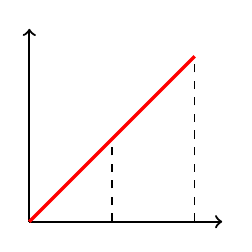
\begin{tikzpicture}[scale=0.7]
\draw[thick,->] (0,0)--(3.5,0);
\draw[thick,->] (0,0)--(0,3.5);
\draw[very thick, red] (0,0)--(3,3);
\draw[dashed] (3,0)--(3,3);
\draw[dashed] (1.5,0)--(1.5,1.5);
\end{tikzpicture}
\end{figure}

Таблица~\ref{tab3} должна иметь номер 3.

\begin{table}[!h]
\caption{Таблица умножения с помощью \texttt{tabu} (фрагмент)}\label{tab3}
\centering
\begin{tabu}{|*{18}{X[c]|}}\hline
-- & 1 & 2 & 3 & 4 & 5 & 6 & 7 & 8 & 9 & 10 & 11 & 12 & 13 & 14 & 15 & 16 & 17 \\\hline
1  & 1 & 2 & 3 & 4 & 5 & 6 & 7 & 8 & 9 & 10 & 11 & 12 & 13 & 14 & 15 & 16 & 17 \\\hline
2  & 2 & 4 & 6 & 8 & 10 & 12 & 14 & 16 & 18 & 20 & 22 & 24 & 26 & 28 & 30 & 32 & 34 \\\hline
3  & 3 & 6 & 9 & 12 & 15 & 18 & 21 & 24 & 27 & 30 & 33 & 36 & 39 & 42 & 45 & 48 & 51 \\\hline
4  & 4 & 8 & 12 & 16 & 20 & 24 & 28 & 32 & 36 & 40 & 44 & 48 & 52 & 56 & 60 & 64 & 68 \\\hline
\end{tabu}
\end{table}

\chapterconclusion

В конце каждой главы желательно делать выводы. Вывод по данной главе~--- нумерация работает корректно, ура!